\section{Design}
\label{sec:design}

% XXX: epidemic: too general, anti-entropy
% more tech details

\begin{figure}
\centering
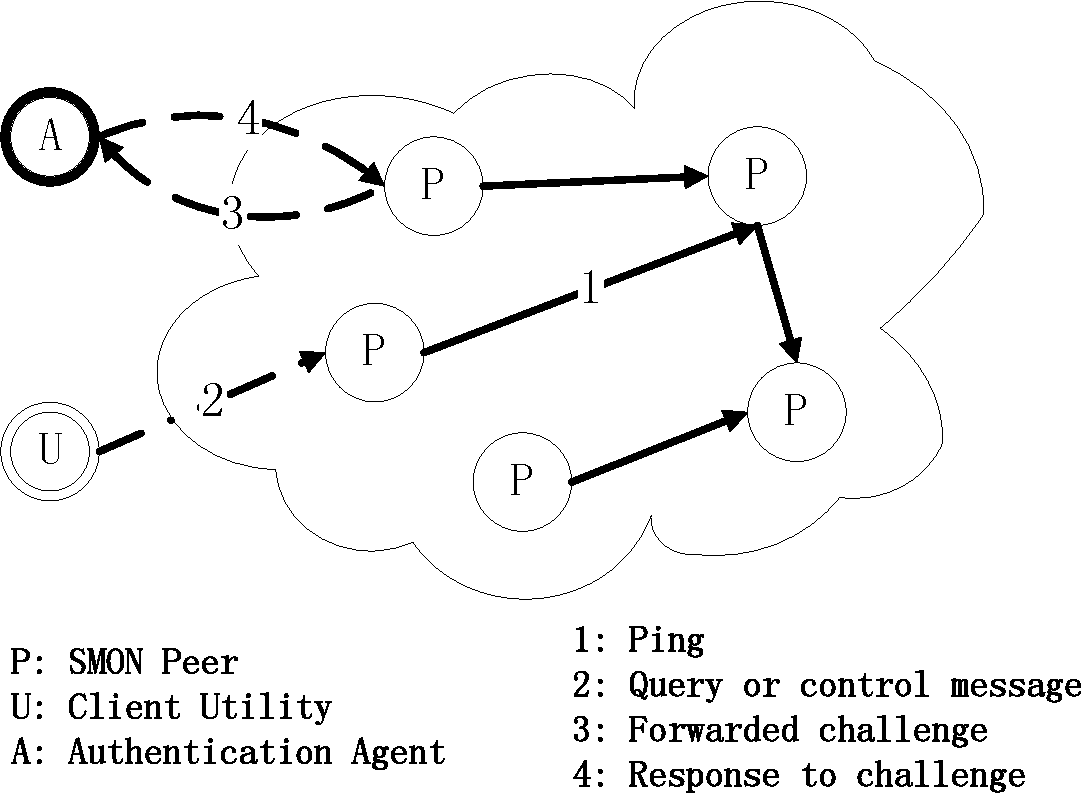
\includegraphics[width=3.0in]{smon_arch}
\caption{SMON system design.  SMON peers monitor each other
by sending ping messages (arrow 1).  User can send query or
control messages using client utility (arrow 2).
Authentication agent resolves authentication challenge from
peers to help them log into other machines automatically
(arrow 3 and 4).
}
\label{fig:smon_arch}
\end{figure}

The design of SMON system is presented in
figure~\ref{fig:smon_arch}.  It consists of three parts: SMON
peers, authentication agent and client utility.

The SMON peers run on a set of target machines where
distributed applications will be deployed. The peers
periodically monitor and maintain each other in their
membership list. The membership list contains machine hosts
names where SMON peers should be deployed and running.
%They will deploy new peers on fresh machines, recover
%failed peers and upgrade themselves to new version. In this
%way, a SMON system can manage itself And automatically. 
With the help of authentication agent, a SMON peer can log
into remote machines automatically to recover failed peers
or deploy new peers. A SMON system can manage a set of
distributed applications. It defines the management semantic
for long running internet services.  User can use the client
utility to instruct SMON on application management. The
utility can also be used to control a SMON system, such as
upgrading it to new version, or query running states of SMON
peers.

% The epidemic algorithm is used extensively in designing
% SMON. A SMON system must hold several distributed invariants
% to run successfully. For example, there should be a SMON
% peer running on all target machines specified by user. The
% epidemic algorithm is applied for the invariant as follows:
% a SMON peer will periodically ping another random peer in
% its membership list, if corresponding pong message is not
% received within timeout, it will try to recover the remote
% peer or deploy a new peer on the remote machine. The
% epidemic algorithm is also used to hold other invariants.
% XXX: for example?

% The SMON peers run on a set of target machines where
% distributed applications will be deployed. Each peer
% maintains the full list of target machines as its membership
% list. The peers monitor and maintain each other using
% epidemic algorithm. A peer periodically chooses a random
% peer and sends it a ping message.  If the pong message is
% not replied within a timeout interval, the remote peer is
% considered as failed. The peer will try to recover the
% failed one by restarting it remotely, or deploying and
% starting a new peer on a fresh machine. Each peer has an
% associated version number. The peers exchanges their version
% numbers epidemically and peers of lower version upgrade
% themselves to the latest versions. The epidemic algorithm
% ensures that the entire SMON system will keep running and
% staying at the latest version eventually.
%
% The authentication agent holds the credential (e.g. private
% key) used to authenticate with the target machines. When
% a SMON peer tries to deploy or restart another peer, it can
% automatically login into the remote machine with the help of
% the agent. The credential is never known to the peers or
% leaked out.
%
% % XXX: quite basic?
% With the help of client utility, user can instruct SMON to
% manage a set of distributed applications. SMON deploys and
% maintains distributed applications using epidemic
% algorithms too. The application management semantic of SMON
% is quite basic. User can extend the management semantic by
% deploying another management system upon SMON.



\comment{
\subsection{Monitor-reaction model}

%The collective behaviour of all peers defines the runtime
%of a SMON system.

\begin{figure}
\centering
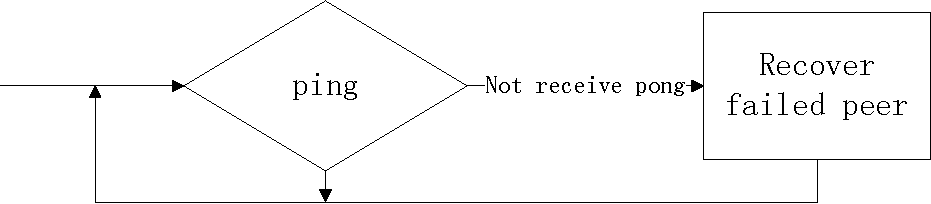
\includegraphics[width=3.0in]{recover}
\caption{recover model}
\label{fig:recover}
\end{figure}

We use a monitor-reaction model to define SMON peer's
behaviors. The model is consistent with and automatically
implements what humans do when maintaining a distributed
system manually. In the model, the ``monitor'' part defines
what status to observe timely, and based on the monitored
result, certain ``reactions'' are performed. Thus, the model
describes a closed-loop control that eliminates human
interventions. For example, a SMON peer will continually ping
other peers to see if they are running. If a pong message is
not received within a predefined timeout interval, we
consider it as failed and try to recover it by login into
the machine and restart it, otherwise, an empty reaction is
performed. The model is shown in figure~\ref{fig:recover}.

The monitor-reaction model can have variations. First, one
model can be nested in the reaction part of another model.
Using previous example, when we know that a peer is failed,
there can be another reason: the machine is crashed and
maybe replaced by a new one with the same host name. To
handle such cases, in the reaction part we need to further
detect whether the machine has a SMON peer installation, if
not, we have to deploy a copy of the peer first. The model
is shown in figure~\ref{fig:recover-nest}.

Second, two or model models can be combined for purposes
such as optimization. For example, SMON peers also exchange
their version numbers and upgrade peers with low version
automatically. This model can be combined with the failure
detector model by piggyback version number within the ping
message. Thus, we can save one RPC call. The combined model
is shown in figure~\ref{fig:combine}.

One peer may implements several models. They run
concurrently and need to be well coordinated. In the upgrade
model, after a new version is retrieved, the peer need to
start the new version and stop itself. Before it execute the
action, other models may be running also. The upgrade model
has to wait others until all of them finish actions part.
The coordination can be implemented by using locks, and in
this case, a reader-writer lock may be more suitable.

The models are required to be stateless in the sense that
the execution of a model is independent with it previous
executions. In this way, the implementation of the model is
as simple as possible and improves peer's reliability.

\note{transaction? the membership list update should be
atomic.}

\note{the combined model looks complex. the reason: 1. for
optimization. 2. we have carefully examined the code and it
runs for a long time without error?}

The models can not be running infinitely. We address this
problem in subsection~\ref{subsec:livetag}.
}

\subsection{Self-management}

A SMON peer runs the pseudo-code in
figure~\ref{fig:peerflow} to manage other peers. We start
from line 5 and explain line 2 and 3 later. A SMON peer will
choose a random machine and send it a ping message (line
5-7). If timeout happens, it will try to deploy a new peer
or recover the failed peer on the remote machine (line
10-16). If the remote peer is running, it will reply with a
pong message. The version number of two peers are
piggybacked in the ping/pong messages and the peer with
lower version will upgrade itself automatically.

We describe how SMON deploys, recovers and upgrades itself
automatically as follow.


\begin{figure}
\centering
\begin{lstlisting}[language=Python,morekeywords={True,False},frame=tb,basicstyle=\small,numbers=right,numbersep=-5pt,numberstyle=\tiny]
while(1):
    if(livetag==False):
        continue

    p = random.choice(membership_list)
    try:
        remote_ver = ping(p, my_ver)
        if(remote_ver > my_ver):
            upgrade_myself()
    except Timeout:
        conn = Connect(p, auth_agent)
        if(conn.is_peer_installed()==True):
            conn.recover_peer()
        else:
            conn.deploy_peer()
        conn.close()

    sleep(WAIT_INTERVAL)
\end{lstlisting}
\caption{SMON peer working flow}
\label{fig:peerflow}
\end{figure}

\subsubsection{Self-deployment}

Given a list of target machines, SMON can deploy itself to
all the machines automatically. At the very beginning, there
is no SMON peer deployed and running. A first peer have
to be deployed and started manually. It then pings other
machines in its membership list and deploys new peers. The
new peers repeat the same ping-and-deploy process. While
there are more SMON peers deployed and running, this process
speeds up exponentially. It is proved that with probability
1 all the reachable machines can be deployed
eventually\cite{Eugster2004}.

%while 1:
%  sleep(T)
%  h = randomchoice(member\_list)
%  try:
%    ping(h)
%  except Timeout:
%    remote\_copy(h, path\_to\_installation\_package)
%    remote\_execute(h, remote\_path\_to\_installation\_package)

%The ping-and-deploy process of a SMON peer implements the
%upper part of the ping model in figure~\ref{fig:combine}.
In detail, a peer $P$ will periodically choose a random
machine $M$ from its membership list and send a ping
message. If a pong message is not received within predefined
timeout intervals, it will start the deployment procedure on
machine $M$. $P$ first authenticates itself with $M$ and
log into $M$ with help of the authentication agent
(described in \ref{subsec:security}), then it copies the
installation package of SMON peer to $M$, starts the package
remotely and logout. The installation package first
checks the integrity of itself (currently using MD5 checksum)
in case of transfer errors during remote copy, then it
installs and starts SMON peer.

There may be failures (e.g. connection corrupted, machine
crashed) at any time when peer $P$ logs
into $M$, copies and starts installation package remotely.
When failure happens, $P$ will just abort the deployment
procedure. $M$ will be chosen by another SMON peer at later
time. It is expected that a new SMON peer will be deployed
on $M$ eventually.

Since peers communicate with each other epidemically, it is
possible that two or more peers try to deploy a SMON peer on
the same machine $M$ simultaneously. This race-condition is
solved without direct coordination among peers. The
installation packages from different peers will be copied to
different directories of $M$ and they will not overwrite
each other. The execution of simultaneously started
installation packages are synchronized using OS provided
synchronization facilities (e.g. lock file). So only one of
the installation will finish and others will abort.  In
solving the problem, some overhead is introduced because
multiple installation packages may be copied, which wastes
network bandwidth and storage resources. Through
mathematical analysis and evaluation on Planet-Lab platform,
it is shown that the overhead is low (a constant value) on
average. Since the size of the installation package is small
(122KB), the overhead can be considered as insignificant.

%It is not easy to define when self-deployment is finished
%globally. Ideally, it is finished when all the target
%machines are reached and deployed with SMON peers.  However,
%considering some machines may be unreachable or shutdown
%from time to time, the `finished-globally' situation is
%rare. Even after a machine is deployed with SMON peer, it
%may crash and be replaced with a new machine with the same
%host name. The peers then have to continue the
%ping-and-deploy process as long as they are live and leave
%the `finish' definition to user. The user can query how many
%or which peers are deployed, and determine whether it is
%appropriate to consider the situation as a finish.

\subsubsection{Self-recovery}

Two kinds of failures may happen and must be handled by
SMON, namely, machine failure and network partition.

When a machine fails, the SMON peer running on it is stopped
also. Other peers know this event through periodic pings and
they will try to recover the failed peer by restarting it
remotely. It is safe to start multiple instances of SMON
peer, but it is idempotent to start only one instance.  In
this way, although false positives are possible in fault
detection, no system churn will be introduced by spurious
recovery.

Network partitions can also be handled by SMON easily. When
network partition occurs, SMON peers are splitted into
several sub-systems, each of which is connected internally.
Implied by epidemic algorithm, each partitioned part will
keep manage itself. When two partitions rejoin, the peers in
different partition will be able to contact and communicate
with each other, leading to the mergence of the whole
system.

% In this way, a peer can choose which action to take based
% on result of a ping message.

\comment{
The SMON system has a global state indicating it is active
or not. When SMON is active, the peer-monitoring component
is enabled. Every SMON peers actively monitor each others
and keep them running as possible as they can. While SMON is
not active, the peer-monitoring function is disable and SMON
acts just like an usual management tools. The active state
is an essential part of SMON system design. Without it, SMON
is just another usual management tool for distributed
applications. If the state is designed as active all the
time, it is a hard problem to stop an active SMON system. If
we try to stop the SMON peers one-by-one, we will noticed
that the stopped peers will soon be restarted by other
peers. And the only way to stop an active SMON system is to
stop all the peers near simultaneously, which is quite hard.
The active state also has an associated version number and
each SMON peer replicates and stores the state with version
locally.  The epidemic algorithm is used to maintain the
state consistently and efficiently among all peers.
}

\subsubsection{Self-upgrade}

As a distributed system, SMON can upgrade itself to a new
version automatically. The upgrade goes online while SMON is
running. User needs not to stop SMON before upgrade.

Each SMON peer has an associated version number and it is
stored persistently with the peer.  A peer will exchange and
compare its version with others epidemically. If there is a
difference, the peer with lower version will retrieve the
installation package from the remote peer and upgrade itself
automatically.

% XXX limit the number of ...?
It is possible that a peer of new version is known by many
peers of old version quickly. To avoid flash crowd, a peer
will limit the number of simultaneous request for retrieving
installation package.

To upgrade the whole SMON system to a new version, user only
has to upgrade one peer to the new version and all the other
SMON peers will converge to the latest version eventually.
The user can upgrade a SMON peer by using the client
utility described in subsection~\ref{subsec:client}.

\comment{
\note{need revise the method, consider the ping interval}
When a SMON peer knows there's a new version of peer, a list of
hosts on which peers with new version are running is gathered
through active detection among peers.  A self-upgrade action is
scheduled to read the list and download the new version. At the
beginning of the self-upgrade process, there would only be a
small number of peers running in new version, but they are known
by a lot of other peers.  If there's not any constraints, a lot
of peers may download from the same host simultaneously. To
prevent that, we use a conservative strategy to control the
self-upgrade action.  The destination is, at average, only a
constant $k$ of peers can download simultaneously from a host.
The algorithm we use does not need any coordination among peers,
and works as follows.  If there are $n$ peers want to download
from the same host. Each of them choose to take the download
action  with probability $k/n$. If the action is not taken, it
will be delayed in the next time. So at average, there will be
only $k$ peers downloading from the same host simultaneously,
and it takes a peer to rerun the action $n/k$ times to select
the same peer.  As peers don't coordinate with each other, they
make a conservative estimation that set $n$ to $N$, the number
of all the peers. The strategy may cause a slow start at the
begin of self-upgrade process because $n$ is far smaller that
$N$. When more peers are upgraded to new version, the upgrade
process would be boosted. If a peer knows $p$ peers of new
version, the probability it choose to not download from any of
them is $q=(1-k/n)^p$ and it takes at average $\frac{1}{1-q}$
tries to choose a host. When $p$ increases, $q$ decreases
quickly and $\frac{1}{1-q}$ will be nearly 1 with large $p$.
}

\comment{
It is important to ensure that communication interfaces for
different versions of SMON peers are consistent. If the condition
is ensured, the whole SMON system can be updated gracefully while
most of peers are running and the system functions well.
Otherwise, the new SMON system can only be deployed after the old
one is stopped.
}

\subsubsection{Disable/enable self-management}
\label{subsec:livetag}

We need mechanism to enable or disable self-management
capability to stop SMON from running. When self-management
is enabled, we cannot stop SMON by shutting down peers
individually.  If a peer is stopped by user, it will be
restarted soon by another peer. The only solution under such
condition is to stop all the SMON peers simultaneously,
which is not feasible at large scale.

We use a boolean variable called \texttt{livetag} to control
epidemic ping among peers. If the value is false, a peer
will stop sending periodic ping message to others and the
whole SMON system stops maintaining itself (line 2-3 in
figure~\ref{fig:peerflow}).
%We can now stop SMON peers one by one.

The \texttt{livetag} variable has an associated version
number and is maintained on each peer distributedly. The
peers exchange \texttt{$<$livetag, version$>$} tuples
epidemically and update the tuple to the latest version.
Note that even the epidemic update of \texttt{livetag} is
controlled by the value of \texttt{livetag}.  When
\texttt{livetag} is false, peers still respond
to incoming messages, so as to
help disseminating the update to \texttt{livetag}.

Suggested by epidemic algorithm, the whole SMON system will
be finally disabled when the \texttt{livetag} value of any
peer is set to false and peers will not send ping messages
to each other. A peer will stop itself from running if no
messages is received for enough long time. In this way, a
SMON system can be shutdown automatically by setting
\texttt{livetag} to false.

% xxx elabrate on random here

% SMON adopts ``crash-only'' design. When SMON peer fails, it
% can be recovered by simply restarting. SMON stores the
%
% self-version, livetag/ver, app name/setting, agent,
% membership ver, k\_e: put to ``combine together''


%\note{the complete execution of a peer}

%\note{peer and installation package, how they coordinate
%when upgrade and deploy.}

%\note{the set of states peer maintains, database?,
%stateless?}


\subsection{Security mechanism}
\label{subsec:security}

SMON's security mechanism should achieve two goals:

\begin{itemize}

  \item Assist peers to authenticate with remote machines so
  as to deploy new peers or recover failed peers.

  \item Authenticate and encrypt access to SMON peers so
  that it will not be misused (e.g. deploying malwares).

\end{itemize}

%SMON peer should be able to login into remote machines
%automatically to deploy new peers or restart failed ones.
%In this process, the authentication credential should be
%keep secret.  \note{here.} It is necessary for different
%SMON peers to authenticate each others and keep the
%communication confidential among them. In addition, when a
%SMON peer deploys new SMON peer on a remote machine, it need
%to authenticate itself with the remote machine to copy
%contents and execute commands (start the installation
%package). The authentication credential is owned by user and
%should be protected confidentially. From another point of
%view, the SMON peers relies upon the authentication
%credentials provided by user to deploy and maintain each
%others automatically in a distributed approach.

We describe how we design security mechanism to achieve the
two goals on Planet-Lab platform and discuss design issues
on other distributed platforms. Planet-Lab uses public-key
system to authenticate access to the platform. A user access
his slice (a set of distributed virtual machines) by using
ssh. The private key is kept in user's computer and the
public key is distributed to all virtual machines of his
slice.

%SMON system is designed for distributed platforms that are
%semi-open---like Planet-Lab or grid, or for proprietary
%ones---such as large machine rooms or data centers. It
%assumes that: 1) the network between machines in a
%distributed infrastructure is not trusted, 2) the users that
%can access the infrastructures are not adversarial, 3) the
%applications running in the infrastructures are not
%adversarial. Based on assumptions above, SMON designed an
%security mechanism which guarantees that 1) communications
%among SMON peers are authenticated and confidential, 2)
%authentication credentials are never leaked. The mechanism
%incorporated in current design supports challenge based
%authentications like public-key authentication scheme, which
%is extensively used.

\begin{figure}
\centering
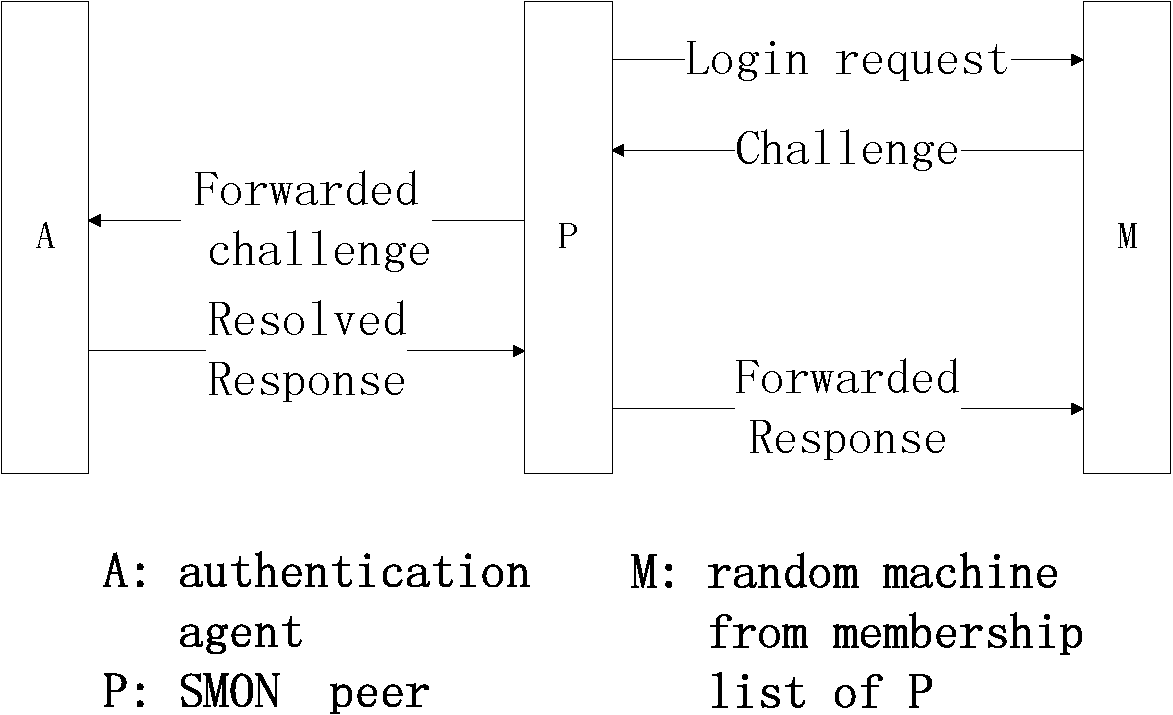
\includegraphics[width=3.0in]{auth}
\caption{Interactions among SMON peer, authentication agent
and a remote machine when the peer logs into the machine.}
\label{fig:auth}
\end{figure}

To achieve above-mentioned two goals, SMON employs an
authentication agent who holds user's private key securely.
As described in figure~\ref{fig:auth}, whenever a SMON peer
needs to login into a machine, it will first connects to the
sshd server of remote machine and sends a login request. The
sshd server will pose an authentication challenge encrypted
by user's public key. The peer will indirect the
authentication challenge from sshd to the agent and reply to
the sshd server with the solved response from the agent. In
this way, a peer can login into any machine in his slice and
the private key is kept secret for all the times. A
symmetric key $K_E$ is shared by all the SMON peers and the
authentication agent. It is used to authenticate with peers
and agent within the same SMON system, and establish
confidential communication channels among them. The shared
key $K_E$ is included within the installation package of the
SMON peer. When a SMON peer is deployed, $K_E$ is deployed
along. Because the deployment is encrypted by ssh, $K_E$ is
not leaked out of the network. $K_E$ is safe to be stored
within user's slice because the storage resource among
virtual machines are well isolated.

\comment{
It is not necessary to keep authentication agent running for
all the time.  When the self-deployment process is finished,
the agent can be closed, and re-open timely for maintenance
purpose.  It is also a security concern to offline
authentication agent to protect user authentication
credentials.
}

The agent should run on machine where user makes sure his
private key is safe. The agent can be also replicated if
required. When a SMON system is deployed at large enough
scales, there can be multiple instances of authenticate
agent for performance considerations. SMON peers can be
directed to their nearest agents by DNS server.

The above agent-based scheme works for challenge-based
authentication method, e.g. password or public-key
authentication, which is commonly used in many systems.
It relies on two key factors:

\begin{itemize}

  \item Using challenge-response authentication mechanisms,
  such as public-key or password authentication.

  \item $K_E$ is safe to be stored with SMON peer.

\end{itemize}

For example, the mechanism can be applied on Amazon EC2
platform and private clusters. For Amazon EC2, user starts
instances of virtual machines based on an AMI (Amazon
Machine Image). The user access his AMI instances using
private key. For private clusters, virtual machine may be not
adopted but users who can access the system are not
adversarial and $K_E$ can be considered safe to stored on
local file systems.

\subsection{Membership}

Each SMON peer maintains a list of machines as its
membership list.  The membership maintenance of SMON system
is different from other distributed systems such as file
sharing, streaming, Content Distribution Network. While
others maintains a list of peers that are currently online,
SMON maintains a list of machines on which there should be
peers running. The failure of SMON peers will not affect the
membership list at all.  The list is specified by user and
should not changes very often. And an important requirement
of SMON is, even when there is only one SMON peer running,
it should be able to know all the target machines where SMON
should be deployed.  The implication is that every running
SMON peer should be able to know the full list of target
machines.

In current design, a simple scheme is used: each SMON peer
will store a replica of the full list of target machines
persistently in compressed format. The list also has an
associated version number. SMON peers exchanges their
membership versions epidemically and update the list. User
can update the membership list to change the set of machines
on which SMON runs.
%To reduce the communication overhead in updating membershit
%list, only the differences between two version are
%propagated during machine list update process.
This scheme is enough for handling machine list containing
even tens of thousands of machines because only the machine
names or IPs are stored in the list.  An estimation shows
that, storing 15000+ machines names in zip format takes
about 100K bytes, which is an acceptable result.

%When membership changes, newly added machines will be
%deployed with new SMON peers. The peer running on removed
%machines will receive the new machine list and find that
%they are not in the list. It will then only reply to
%incoming messages to help spreading membership changes. And
%it will stop maintaining any SMON peer.  After most peers
%update their membership list, the peers in removed machines
%will kill themselves after they don't receive any messages
%for enough long time.

\subsection{Application management}

SMON can manage one or more distributed applications. The
management semantic is defined in the following four
dimensions, which is a general framework for describing
application management requirements.

\begin{itemize}

  \item resource requirement: different applications put
  various demands on computing resources, such as CPU load,
  free disk space and memory, network bandwidth and latency,
  etc. Besides from characteristics on current resource
  usage, user may be also interested in resource availability
  and reliability which can be inferred by summarizing
  historic data. The management system should find best set
  of resources as described in specification.

  \item deployment: The management system follows
  instructions given by user to copy, unpack and install
  applications on acquired resources. The management system
  should also support a variety of file transfer mechanisms.

  \item synchronization: distributed applications may work
  in multi-phases, such as scientific parallel programs.
  The management system should have barrier mechanism to
  execute application workflow in steps.

  \item maintenance and recovery: While application is running,
  the resource usage may vary and failures of different
  levels may happen. The management system should monitor
  dynamic resource conditions and recover applications from
  failure as soon as possible.

\end{itemize}

Two common kinds of distributed applications are long
running internet services and grid style computation
programs. The management requirements are summarized in
table~\ref{fig:app-man-req}.

\begin{table*}
\small
\centering
\begin{tabular}{|l|p{5cm}|p{5cm}|}

\hline

 & long running internet service & grid style computation
 program \\

\hline

resource requirement & prefer resources with good
reliabilty to provide sustained performance for long time
(may be years) & prefer
 resources with huge computation and storage capabilities,
 reliability is required only when computations are running
 (usually short, e.g. days) \\

\hline

deployment & platform specific & platform specific \\

\hline

synchronization & peers can be started independently, and there
is no constraints on peers starting order &
parallel computation programs must be started nearly
simultaneously, and the computation may have multiple
phases.\\

\hline

maintainance and recovery & failure of a single peer can be
handled gracefully, and the peer can be restored to maintain
sustained performance &
failure of a single computation program may lead to failure
of whole computation.\\

\hline

\end{tabular}
\caption{Comparison of management requirements for long
running internet services v.s. grid style computation
programs.}
\label{fig:app-man-req}
\end{table*}


SMON support management semantic for long running internet
services. Such services include file
sharing, streaming,
Content Distribution Network, etc. These
services may run for months or years and must robust to a
variety of failures. After the services are deployed, the
application peers (shortened as ``app-peer'') can be started
independently without particular sequences. The app-peers
organize themselves into structured or random overlays and
handles network churns and failures. When an app-peer fails,
the overlay can re-organize itself. The failed app-peer
should be restored as quickly as possible to maintain
service availability and performance.

To manage a long running service, SMON will deploy the
application to a set of machines. It is up to the user to
decide the machines list using resource discovery services.
The application peers are started by SMON once they are
deployed without synchronization. A SMON peer will monitor
and maintain app-peer in the same machine. When an app-peer
is failed, it will be restarted for recovery.

\begin{figure}
\centering
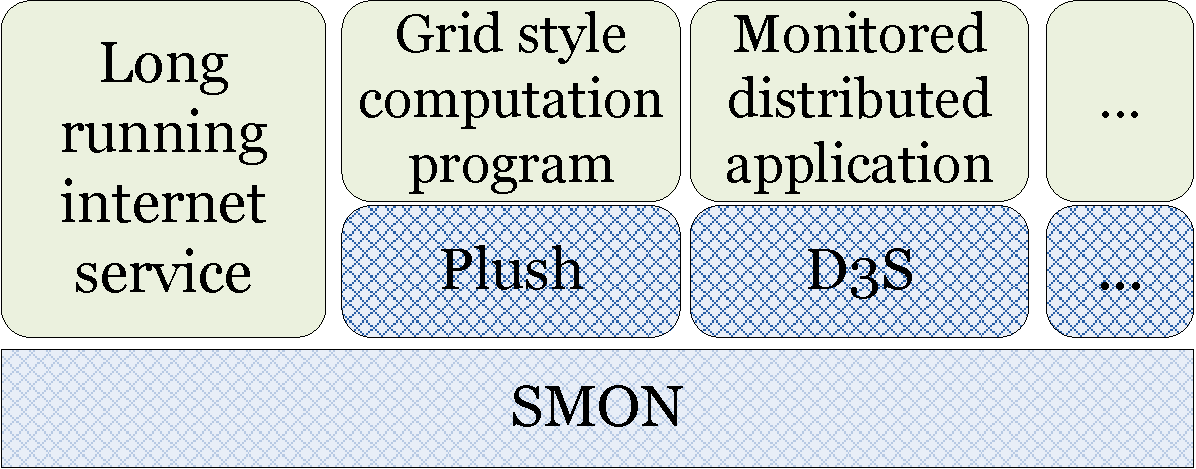
\includegraphics[width=3in]{extend_smon}
\caption{Enrich management semantic by deploying other
management systems upon SMON.}
\label{fig:extend_smon}
\end{figure}

Because distributed application management systems fit in
the catalogue of long running services, we can easily enrich
the management semantic by deploying another management
system upon SMON. In this way, the management functionality
can be ``extended'' greatly, while the combined management
system keeps self-management capability. For example, we can
layer Plush~\cite{Albrecht2007} upon SMON to manage grid
style computing programs as shown in
figure~\ref{fig:extend_smon}. Plush provides barrier support
for dividing computations in phases, manage application in
coordinated approach or on a sebset of nodes. Or we can layer
D3S~\cite{Liu2008} on SMON to monitor and debug correctness
of distributed applications as a set of predicates, which
are defined on runtime states of application processes on
many machines.

% To enrich more advanced management semantic, user can first
% deploy another management or monitoring system on top of
% SMON. The ``combined'' management system still preserve
% self-managment capacity. For example, D3S~\cite{Liu2008} is
% a monitoring tool which uses distributed predicates to
% monitor application's internal states. It exports
% application's states using instrumentation~\cite{Guo2008}
% and calculates user specified predicates on global
% snapshots. Whenever a predicate is false, the event is
% reported. User can delay D3S on top of SMON and define
% safety or liveness predicates to check application states in
% detail.

SMON deploys applications using epidemic algorithm.  An
application is uniquely identified by its name.
Periodically, a SMON peer $A$ will choose one locally
deployed application and notify a random peer $B$ with the
application name. If $B$ knows an un-deployed application,
it will try to retrieve the installation package from $A$
and install the application. If the retrieve fails, $B$ will
just wait for the next notification. The epidemic approach
ensures that an application can be pushed out to all SMON
peers eventually.

%There is a set of implemented RPC calls for control and
%monitoring of managed applications.

%Each of the managed application peers has an
%associated version number.  The version numbers of
%application peers are maintained by managing SMON peers. The
%similar epidemic algorithm is used for keeping application
%peers up-to-date. A trick used in application management is,
%when an application peer has not been deployed on a machine
%yet, its version number is set to 0.0, which is smaller than
%any real version numbers. In this way, application
%deployment problem is turned to the application update
%problem.

After application is deployed and started, it is monitored
and maintained by SMON peer in the same machine. SMON reads
application specification for management options. User can
specify application's default running state and change the
setting using client utility provided by SMON.

The application's running states can be:

\begin{itemize}
  \item Online: the application will be restarted once
  stopped.
  \item Offline: the application will be stopped.
  \item Ignore: the application will be started for the
  first time and its state will not be monitored after
  that.
\end{itemize}

In the specification, user should specify three scripts to
start, stop and restart the application. The restart script
is called to recover the failed processes, and may include
clean up steps before application is restarted.

A SMON peer may report the application states to a central
server timely if specified. And whenever the application
state changes, the SMON peer will report the changes
immediately.

% It is obvious that the application monitoring and
% maintenance semantic provided by SMON is very basic. It
% only considers whether an application is running, without
% further monitoring liveness or safety states. This
% is enough for maintaining long running services whose peers
% should be running as long as possible.

% appname, state, report machine, start/stop/restart binary,
% report interval, report url (appname=xxx, status=xxx) (or
% report binary?)
%
% include/exclude machine?
%
% bin/conf/data
%
% state can be modified per machine, but has an initial value.

\subsection{Client utility}
\label{subsec:client}

A client utility is provided for user to control SMON. The
communication between the utility and any peers is
authenticated and encrypted by the share key $K_E$. To
deploy SMON, the utility will copy the installation package
of SMON peer to a machine and start the package, then SMON
will deploy itself automatically. To upgrade SMON, the
utility mimics itself as a SMON peer and notifies a random
SMON peer that a new version available.  The peer will then
retrieve the installation package from utility's machine and
upgrade itself. Then SMON will be upgraded.  Similarly, the
utility can notify a random peer to install an application,
update the member list and enable or disable self-management
capability of SMON. The latest version numbers of SMON peer,
membership list and \texttt{livetag} are stored locally on
user's machine.  User can query any SMON peer with the help
of the utility.

%The query RPCs are summarized below. \note{xxx}

%smon: version
%app: set/get status


\comment{
SMON, live? version?

query app, live?

update version

install application

set/query \texttt{livetag},

maintain version number of SMON and live tag
}

\comment{
To improve reliability, the one-hop source
routing\cite{Gummadi2004} algorithm is implemented. When the
utility failed to communicate directly with a peer, it
randomly selected $k$ ($k=4$ in current design) other peers
for redirecting the message.  This feature is useful for
managing large number of machines. We implement this mechanism
because we notice a lot of connection problems caused by
name resolution error. It happens between our laptop and
Planet-Lab machines, and also among some Planet-Lab machines.  In
the experiment, we noticed a machine cannot connect to other
two machines because of name resolution error for more than one
day.  But through one-hop source routing, they can
communicate without problem. This feature is useful for
users to control or monitor machines at large scale. As the
user control or monitor other machines through a peer as proxy,
one-hop source routing can increase the number of connected
peers.
}

% vim:foldmethod=marker:textwidth=60
